\documentclass[11pt,a4paper]{article}
%%%%%%%%%%%%%%%%%%%%%%%%% PACKAGE starts HERE %%%%%%%%%%%%%%%%%%%%%%%%
\usepackage{graphicx}
\usepackage[labelfont=bf]{caption}
\usepackage{microtype}
\captionsetup[table]{name=Table}
\captionsetup[figure]{name=Figure}
\usepackage{tabulary}
\usepackage{fancyhdr}
\usepackage{placeins}
\usepackage[all]{xy}
\usepackage{tikz}
\usepackage{verbatim}
%% Sets page size and margins
\usepackage[a4paper,top=3cm,bottom=2cm,left=3cm,right=3cm,marginparwidth=1.75cm]{geometry}
\usepackage[colorlinks=true, allcolors=blue]{hyperref}
\hypersetup{
    colorlinks,
    linkcolor={red!50!black},
    citecolor={blue!50!black},
    urlcolor={blue!80!black}
}
\usepackage{subcaption}
\usepackage{multirow}
\usepackage{psfrag}
\usepackage[T1]{fontenc}
\usepackage{lmodern}
\usepackage[scaled]{beramono}
% Enable inserting code into the document
\usepackage{listings}
\usepackage{xcolor} 
\usepackage{lipsum}
\usepackage[nodayofweek]{datetime}
%% Language and font encodings
\usepackage[english]{babel}
\usepackage[utf8x]{inputenc}
\usepackage[T1]{fontenc}
%% Useful packages
\usepackage{amsmath}
\usepackage{graphicx}
\usepackage[colorinlistoftodos]{todonotes}
% custom color & style for listing
\definecolor{codegreen}{rgb}{0,0.6,0}
\definecolor{codegray}{rgb}{0.5,0.5,0.5}
\definecolor{codepurple}{rgb}{0.58,0,0.82}
\definecolor{backcolour}{rgb}{0.95,0.95,0.92}
\definecolor{LightGray}{gray}{0.9}
\lstdefinestyle{mystyle}{
	backgroundcolor=\color{backcolour},   
	commentstyle=\color{blue},
	keywordstyle=\color{codegreen},
	numberstyle=\tiny\color{codegray},
	stringstyle=\color{codepurple},
	basicstyle=\ttfamily\footnotesize,
	breakatwhitespace=false,         
	breaklines=true,                 
	captionpos=b,                    
	keepspaces=true,                 
	numbers=left,                    
	numbersep=5pt,                  
	showspaces=false,                
	showstringspaces=false,
	showtabs=false,                  
	tabsize=2
}
\lstset{style=mystyle}
\captionsetup[lstlisting]{labelfont=bf}
\renewcommand{\lstlistingname}{Code}
%%%%%%%%%%%%%%%%%%%%%%%%% PACKAGE ends HERE %%%%%%%%%%%%%%%%%%%%%%%%

%%%%%%%%%%%%%%%%%%% using theorem style %%%%%%%%%%%%%%%%%%%%
\newtheorem{thm}{Theorem}
\newtheorem{lem}[thm]{Lemma}
\newtheorem{defn}[thm]{Definition}
\newtheorem{exa}[thm]{Example}
\newtheorem{rem}[thm]{Remark}
\newtheorem{coro}[thm]{Corollary}
\newtheorem{quest}{Question}[section]

%%%%%%%%%%%%%%%%%% Settings of the page %%%%%%%%%%%%%%%%%%%
\pagestyle{fancy}
\lhead{Francesco Brischetto}
\rhead{ Student Number: 958022\qquad\thepage}
\cfoot{\textbf{Geometry-based shading for shape depiction enhancement, an implementation}}
\renewcommand{\headrulewidth}{0.4pt}
\renewcommand{\footrulewidth}{0.4pt}
%% Change table of contents title
\addto\captionsenglish{
	\renewcommand{\contentsname}%
	{Table of Contents}%
}
%%%%%%%%%%%%%%  Shortcut for usual set of numbers  %%%%%%%%%%%

\newcommand{\N}{\mathbb{N}}
\newcommand{\Z}{\mathbb{Z}}
\newcommand{\Q}{\mathbb{Q}}
\newcommand{\R}{\mathbb{R}}
\newcommand{\C}{\mathbb{C}}
\setlength\headheight{14pt}

%%%%%%%%%%%%%%%%%%%%%%%%%%%%%%%%%%%%%%%%%%%%% BODY DOCUMENT %%%%%%%%%%%%%%%%%%%%%%%%%%%%%%%%%%%%%%%%%%%%%
\begin{document}
	\begin{titlepage}
	
	\newcommand{\HRule}{\rule{\linewidth}{0.5mm}} % Defines a new command for the horizontal lines, change thickness here
	
	%----------------------------------------------------------------------------------------
	%	LOGO SECTION
	%----------------------------------------------------------------------------------------
	\centering
	
\includegraphics[width=4cm]{Images/logo.png}\\[1cm] % Include a department/university logo - this will require the graphicx package
	
	%----------------------------------------------------------------------------------------
	
	\center % Center everything on the page
	
	%----------------------------------------------------------------------------------------
	%	HEADING SECTIONS
	%----------------------------------------------------------------------------------------
	
	\textsc{\LARGE Project Report}\\[1.5cm] 
	\textsc{\Large Geometry-based shading for shape depiction enhancement}\\[0.3cm] 
	\textsc{\large An Implemetation}\\[0.5cm] 
	
	%----------------------------------------------------------------------------------------
	%	TITLE SECTION
	%----------------------------------------------------------------------------------------
	\makeatletter
	\HRule \\[0.4cm]
	{ \huge \bfseries Real-Time Graphics Programming Project}\\[0.4cm] % Title of your document
	\HRule \\[1.5cm]
	
	%----------------------------------------------------------------------------------------
	%	AUTHOR SECTION
	%----------------------------------------------------------------------------------------
	
	\begin{minipage}{0.4\textwidth}
		\begin{flushleft} \large
			\emph{Author:}\\
			Francesco Brischetto
		\end{flushleft}
	\end{minipage}
	~
	\begin{minipage}{0.4\textwidth}
		\begin{flushright} \large
			\emph{Submitted to:} \\
			Dr. Davide Gadia \\[1.2em] 
		\end{flushright}
	\end{minipage}\\[0.5cm]
	~
	\begin{minipage}{0.85\textwidth}
		\begin{flushleft} \large
			\emph{Student Number:}\\
			958022
		\end{flushleft}
	\end{minipage}
	\\[2cm]
	\makeatother
	
	
	%----------------------------------------------------------------------------------------
	%	DATE SECTION
	%----------------------------------------------------------------------------------------
	\newdate{date}{07}{03}{2022}
	{\large \displaydate{date}}\\[4cm] % Date, change the \today to a set date if you want to be precise
	
	\vfill % Fill the rest of the page with whitespace
	
\end{titlepage}
	\pagebreak	
	\tableofcontents
	\pagebreak
	\section*{Executive Summary}
\addcontentsline{toc}{section}{\numberline{ii}Executive Summary}

This project report describes the realization and implementation decisions of the shading technique proposed in \cite{referencePaper}. \newline 
The paper's goal is to describe an approach for \textbf{enhancing shape depiction} of 3D objects on \textbf{Non-Photorealistic Rendering (NPR) shading models} using \textit{local geometry}. \newline
The approach described provides \textbf{time-efficiency}, to make it usable in \textit{interactive application}, without any constraints on the choice of material or illumination model. 
\newline The proposed method is inspired by \textbf{Normal Enhancement} and \textbf{Radiance Scaling} Shading approach and it tries to combine the advantages of both techniques while, also, relaxing their constraints. \newline
The overall goal of my project is to implement some of the newest techniques in NPR as well as coding some of the most famouse ones.
	\section{Introduction}
The advent of Computer Graphics has \textbf{not replaced artists}. Many non-photorealistic rendering techniques have focused on depicting shape through shading that \textit{mimic hand-drawn illustration} but NPR models still \textbf{lack in expressive power}. \newline
The proposed technique should \textit{correlate} the enhancement functionalities to \textbf{surface feature variations}. To achieve this result, the paper \cite{referencePaper} starts from analyzing two existing techniques that either perturbates the surface normal as in \textbf{Normal enhancement} or alterates reflected radiance based on local surface information as in \textbf{Radiance scaling}. \newline
However, both of those methods have some limitations: \newline 
Normal enhancement operators are \textit{restricted} on specific types of material and illumination models, and they are \textbf{not able to enhance} some important geometry features such as \textbf{concavities} and \textbf{convexities}. In contrary, Radiance scaling overcomes those limitations but (expecially in NPR shading) tends to mask subtle shading variations and hence \textbf{reduce effectiveness} of the overall technique. \newline
The proposed techinque's goal is to \textit{reformulate} NPR shading models with respect to \textbf{geometry surface features} combining the advantages of Normal enhancement and Radiance scaling while also \textbf{relaxing their constraints}. \newline
The enhancement is achieved in two ways. First, by \textit{modifying the surface normal} using a simple high-frequency enhancement operation. Second, by correlating reflected lighting intensity to \textbf{surface curvature} using a new scaling function. \newline
In this way, we can achieve enhacement in diffierent extent, allowing users to produce more desirable enhacement results.

\subsection{Project Overview}
In this project I implemented all the shading models used in \cite{referencePaper} :\newline
\textbf{Blinn-Phong}, \textbf{Cartoon} and \textbf{Gooch} as well as their \textbf{enhanced version}, following the reformulation of the \textit{reflectance radiance equation} described in paragraphs 6.1, 6.2 and 6.3 of \cite{referencePaper}. \newline Contextually, I realized also all the needed \textbf{helping operators}, such as \textit{normal smoothing}, \textit{sharpening} and \textit{curvature} calculation. Lastly, I realized other \textit{subroutines} to better visualize the differences between normal and enhanced normal, as well as curvature and enhanced curvature (that uses enhanced normal). \newline
A list of all the usable subroutine in the project can be seen in \textbf{Figure \ref{fig:all_subroutines}}.

\begin{figure}[h]
	\centering
	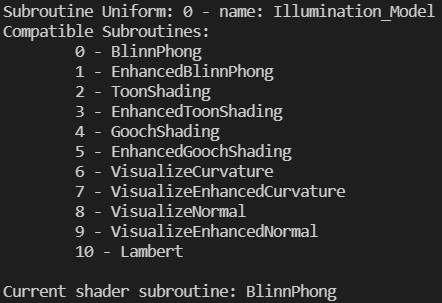
\includegraphics[width=0.5\textwidth]{Images/all_subroutines.jpg}
	\caption{All subroutines available in the project}
	\label{fig:all_subroutines}
\end{figure}
	\section{Geometry-based shading Approach}
The key of this approach is  \textit{incorporating surface curvature} information into shape depiction enhancement technique. This is done with multiple steps:
\begin{enumerate}
	\item  \textbf{3D Shape Descriptor:} 3D Object surface shape is analyzed using the shape descriptor. \textbf{Curvature computation} extracts salient surface features. Tts contribution can be controlled using some parameters.
	\item \textbf{Geometry-based Shading:} the surface normals are \textit{smoothed} or \textit{sharpened} to attenuate or exaggerate the surface depiction; Then, the \textbf{reflected lightning intensity} is scaled using also surface curvature previously calculated.
	\item \textbf{Rendering:} This shading technique is applied to various \textbf{non-photorealistic rendering styles}, reformulating the reflected radiance equation in a way that takes the enhanced shading into account.
\end{enumerate}
In \textbf{Figure \ref{fig:method}} the rendering pipeline is graphically illustrated.
\begin{figure}[h]
	\centering
	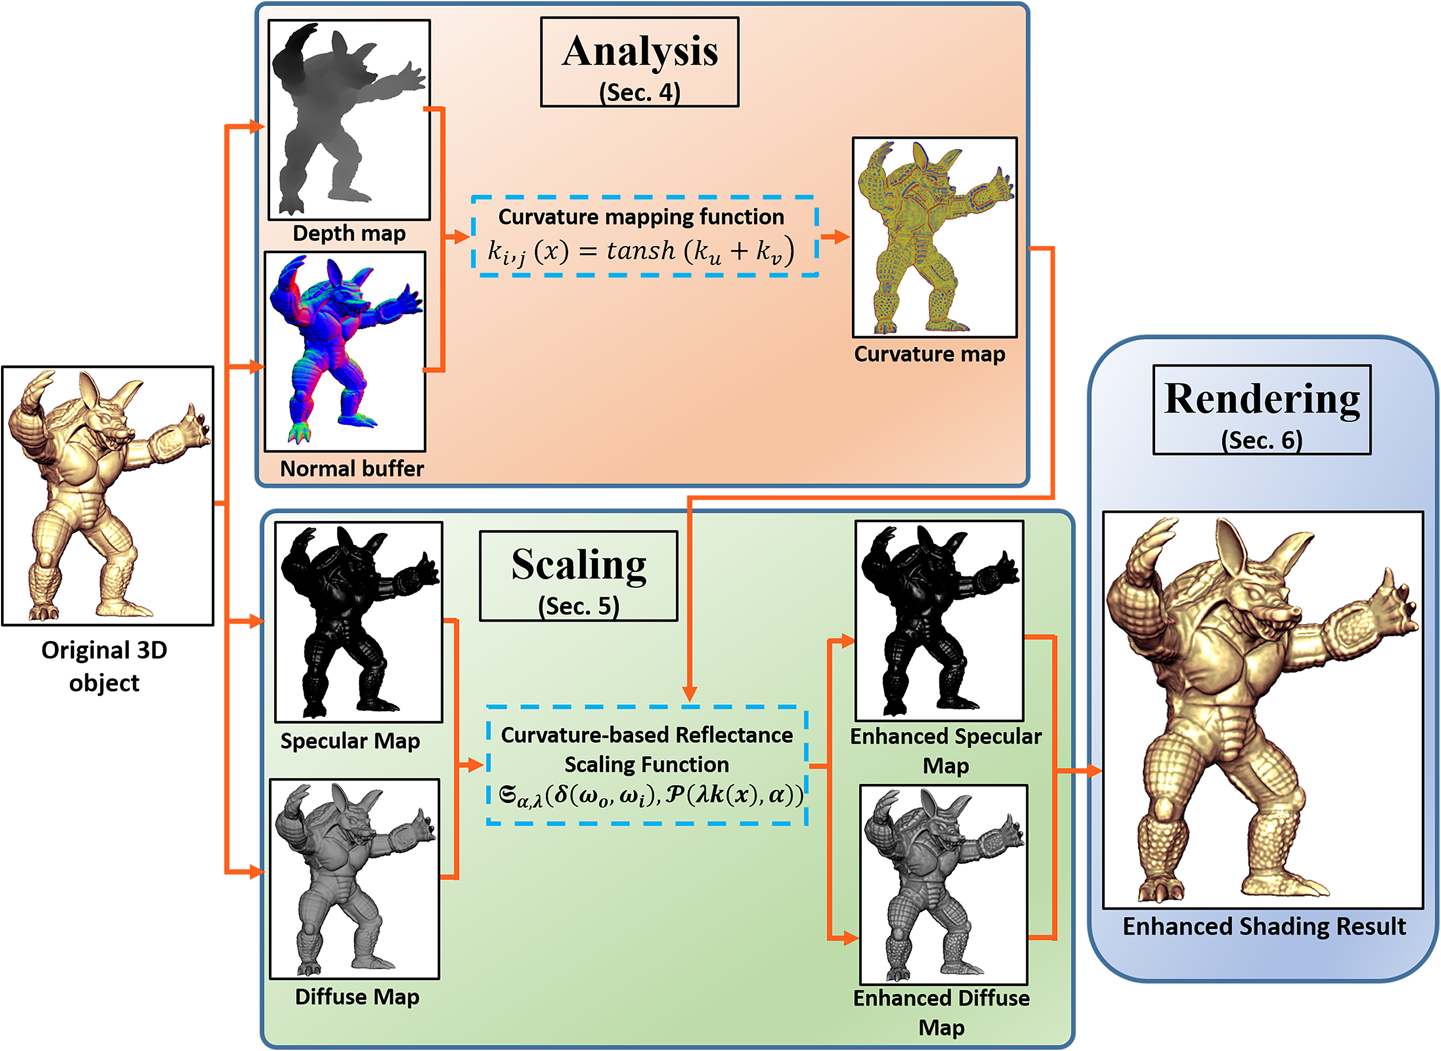
\includegraphics[width=0.75\textwidth]{Images/method.png}
	\caption{The rendering pipeline of the paper's approach. It combines estimating the surface curvature, scaling the reflected lighting and rendering the NPR result}
	\label{fig:method}
\end{figure}
	\section{Design and Implementation}
In this chapter, I will cover all the implementation choices that I made during the realization of the project. Some of the operations described in the paper \cite{referencePaper} where not clearly specified so I was forced to take some implementation decisions and use the paper as a guideline. Moreover, some operations where too general and customizable so I tried to simplify it to make the project simpler. \newline
	Code-wise, My project started from the code version \textbf{lecture03a} that we saw during lectures. I also used 3 standard models in Computer Graphics for testing, downloaded from \textbf{Stanford} website\footnote{\url{http://graphics.stanford.edu/data/3Dscanrep/}}: \textit{Bunny}, \textit{Armadillo} and \textit{Dragon}.
\subsection{Normal Enhancement Operators}
The paper \cite{referencePaper} describes two types of normal variations: \textit{smoothing} and \textit{sharpening}. Those two kind of enhancement operators works on the high-frequency components of the surface normal. Smoothing reduces those components, while Sharpening increase them. 
\subsubsection{Normal Smoothing Operator Implementation}
To calculate smoothed surface normal I started from this idea\footnote{\url{https://www.reddit.com/r/opengl/comments/6976lc/smoothing_function_for_normals/}}. The implementation of normal smoothing operator was done in model\char`_v1 file, while \textit{processing the Assimp mesh} in order to obtain an \textit{OpenGL mesh}. I created a \textbf{new position in the vertex attribute}, that stores smoothed normal. \newline
In this way, data can be loaded in vertex shader by simply add the line in \textbf{Code \ref{code:vert_smoothing}}. \newline
The smoothing normal computation is done for each vertex. I \textbf{initialized} it to vector zero. Then, I \textbf{computed face normal} for each face of the mesh and I \textit{added} it to each vertex of the face. Finally, for each vertex, I \textbf{normalized the result} of this sum. \newline
By doing so, I implicitely consider the \textit{kernel} of convolution as the \textit{smallest one}, considering as \textbf{neighbourhood} only the faces that share the same vertex. I also implicitely defined the \textit{$\sigma$} parameter, found in Equation 5 of 4.2.1 chapter of \cite{referencePaper} that \textit{weights} this operation as \textit{1}. This greatly \textbf{simplifies} computation and code while maintaning the same \textit{intent} as the original paper. The added lines of code are showed in \textbf{Code \ref{code:smoothing_model}}.
\begin{lstlisting}[language=C++, caption=Smoothed normal loaded in vertex shader,label={code:vert_smoothing}]
layout (location = 2) in vec3 sm_normal;	
\end{lstlisting}
\begin{lstlisting}[language=C++, caption=Smoothed normal computations added in processMesh method of model\char`_v1 file ,label={code:smoothing_model}]
	for(GLuint i = 0; i < mesh->mNumVertices; i++)
	{
		Vertex vertex;
		...
		vertex.Sm_Normal = glm::vec3();
		...
	}
	// For each face, I calculate the face normal and I add to the vertices' normal used by the face. Finally, I normalize the normal to obtain the smoothed surface normal.
	for ( int i = 0; i < indices.size(); i += 3 )
	{
		// I Compute the face normal using triangleNormal method, that computes normal starting from triangle points
		glm::vec3 faceNormal = glm::triangleNormal(
		vertices[indices[i]].Position,
		vertices[indices[i+1]].Position,
		vertices[indices[i+2]].Position);
		
		
		
		// I add face normal to each of the 3 vertex normal of the face
		for ( int j = 0; j < 3; j++ )
		{
			vertices[indices[i+j]].Sm_Normal += faceNormal;
		}
	}
	for (auto &v : vertices)
	{
		// Normalizing the vectors accumulating face normals to obtain the smoothed surface normal
		// NOTE: Sigma parameter, found in Equation 5 of 4.2.1 chapter of the reference paper ( to control the quantity of convolution kernel used ) is implicitely 1.
		v.Sm_Normal = glm::normalize(v.Sm_Normal);
	}	
\end{lstlisting}
\subsubsection{Normal Sharpening Operator Implementation}
Normal Sharpening operator is implemented in \textbf{fragment shader} and uses the smoothed normal previously described and passed to the \textit{vertex shader}. \newline
In vertex shader, I apply \textit{normal Matrix transformation} before passing them to the fragment shader as showed in \textbf{Code \ref{code:vert_sharpening}} . \newline
In fragment shader, I calculate the \textbf{mask} by subtracting the original normal vector with its smoothed version. Then, I add the mask multiplied by a \textbf{scaling factor} $\lambda$ to the normal vector, with a typical process called \textbf{unsharp masking} as described in Equation 6 of 4.2.2 chapter of \cite{referencePaper}. Finally, I normalize the result. \newline
The \textbf{Code \ref{code:frag_sharpening}} is added to the fragment shader to implement this process.
\begin{lstlisting}[language=C++, caption=Transformation applied to smoothed normal in vertex shader,label={code:vert_sharpening}]
	vSMNormal = normalize( normalMatrix * sm_normal );
\end{lstlisting}
\begin{lstlisting}[language=C++, caption=Calculation of normal sharpening operator in fragment shader,label={code:frag_sharpening}]
	// Computing the mask for Unsharp Masking
	vec3 mask = vNormal - vSMNormal;
	// calculating enhanced Normal using the Unsharp Masking technique. This is defined, in the reference paper, in equation 6 of chapter 4.2.2
	vec3 eNormal = vNormal + lambda * mask;
	// normalization of the per-fragment enhanced normal 
	vec3 N_I = normalize(eNormal);	
\end{lstlisting}
A Comparison between normal vector and enhanced normal vector (through sharpening) is showed in \textbf{Figure \ref{fig:normal_comparison}} that shows two subroutines created in the project.
\pagebreak
\begin{figure}[h]
	\centering
	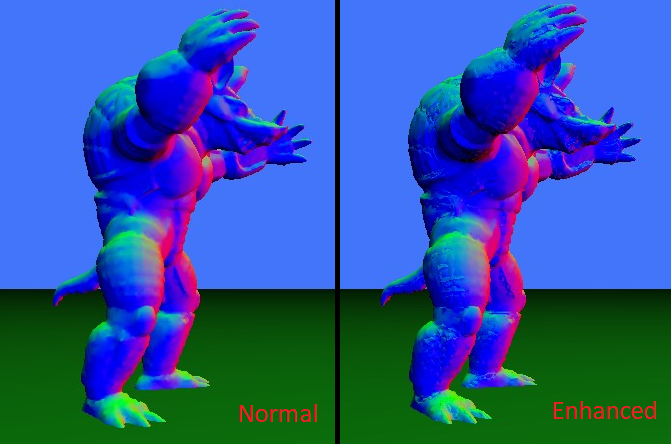
\includegraphics[width=0.8\textwidth]{Images/normal_comparison.png}
	\caption{Comparison between normal and enhanced normal vector (through sharpening)}
	\label{fig:normal_comparison}
\end{figure}
\subsection{Curvature Analysis}
Curvature analysis is another key point of the technique described in \cite{referencePaper}. \newline
However, curvature calculation was not so clear and straightforward in the paper because they introduced the \textbf{second fundamental tensor} and the computation of \textbf{Hessian of depth field} by differentiating the gradient with a \textit{Sobel filter}. \newline
The approach implemented in my project, instead, is simpler. It starts from here\footnote{\url{https://madebyevan.com/shaders/curvature/}} and considers \textbf{screen-space normals of neighbouring} fragments as well as \textbf{depth of the current fragment} to compute a curvature value.
\subsubsection{Screen Space Surface Curvature Implementation}
Surface curvature is computed in screen space, using OpenGL partial derivatives functions TODO.
\subsection{Non-Photorealistic Rendering shading styles}
As previously said, the goal of \cite{referencePaper} is to render 3D objects \textit{without any constraint} on the
choice of material or illumination, while taking into consideration the way of Geometry-based Shading technique that \textit{enhances the lighting} at each surface point. \newline
To achieve this, the authors of \cite{referencePaper} demonstrated their approach with three different \textbf{non-photorealistic shading styles}: \textit{Blinn-Phong Shading}, \textit{Cartoon shading} and \textit{Gooch} Shading. For each of those styles, they \textbf{adapted} their technique by choosing properly an \textbf{intensity mapping} function $\delta$ to be used in the reflected radiance equation.
\pagebreak
\subsubsection{Enhanced Blinn-Phong Shading implementation}
In the context of non-photorealistic rendering, it is common to make use of \textit{simple shading models} such as Blinn-Phong shading model. \newline
Geometry-based shading technique can alter surface shading to enhance surface fine-scale \textbf{geometric details} in a non-photorealistic manner. This process is performed by incorporating enhanced surface normal and surface curvature measure into Blinn-Phong.
\newline
As \textbf{intensity mapping} function \cite{referencePaper} choosed $\delta_j$ = $\rho_j$, where j $\in$ \{ a, d, s \} iterates over the components of Blinn-Phong's shading models: ambient, diffuse and specular. \newline
With this approach, using a single light, the lightning equation becomes:
\begin{equation}
	L_r(x,\omega_o) = \sum_j \rho_j(\omega_o,l) \mathcal{G}_j(x,\omega_o,l) L_j(l)
\end{equation}
In this equation, l is the direction of the light source at point x, $L_j$ corresponds to the light intensity of each component, $\rho_a$ = 1, $\rho_d(l)$ = $(n'\cdot  l)$, $\rho_d(s)$ = $(n'\cdot  r)^f$; \newline
$n'(x)$ is the \textbf{enhanced surface normal}, r is the reflection direction, f is the shininess parameter and $\mathcal{G}_j(x,\omega_o,l)$ corresponds to the \textbf{Curvature-based Reflectance Scaling Function}. \newline
In particular, $\mathcal{G}_j$ is computed as:
\begin{equation}
	\mathcal{G}_j(\delta, P) = \frac{\delta}{e^P (1-\delta) + \delta}\quad\mathrm{where}\quad  P_{\lambda,\alpha}(k) = pow(\lambda |k|, \alpha)
\end{equation}
In this equation, $P_{\lambda,\alpha}$ is the \textbf{curvature mapping} function; its magnitute and strength are controlled using two parameters $(\lambda,\alpha)$; $\delta$ corresponds to the previously declared \textbf{intesity mapping} function.\newline
Code-wise, I started from Blinn-Phong implementation, already present in \textbf{lecture03a} repository, and modified it as we can see in \textbf{Code \ref{code:blinn-phong-enhanced}}, introducing all the previously listed functions. \newline
\begin{lstlisting}[language=C++, caption=Enhanced Blinn-Phong subroutine and Curvature-Based Reflectance scaling function implemented in fragment shader,label={code:blinn-phong-enhanced}]
	
	
	
	// Curvature-Based Reflectance Scaling Function
	float Lr(float curvature_value, float delta)
	{
		// We apply the curvature mapping function that uses lambda and alpha parameters to apply non-linear mapping
		float P = pow (lambda * abs(curvature_value), alpha);
		// Uses as intensity mapping function the second parameter, delta
		// This function maps intensity mapping and curvature mapping functions in the reflectance radiance equation
		// This aims to correlate the reflected lightning intensity to surface curvature
		float G = delta / ( exp(P) * ( 1 - delta ) + delta );
		return G;
	}













	// a subroutine for the Enhanced Blinn-Phong model using Shape Depiction Enhancement based on local Geometry 
	subroutine(ill_model)
	vec3 EnhancedBlinnPhong()
	{
		// Computing the mask for Unsharp Masking
		vec3 mask = vNormal - vSMNormal;
		// calculating enhanced Normal using the Unsharp Masking technique. This is defined, in the reference paper, in equation 6 of chapter 4.2.2
		vec3 eNormal = vNormal + lambda * mask;
		// normalization of the per-fragment enhanced normal 
		vec3 N_I = normalize(eNormal);
		// calculating curvature value using enhanced normal
		float curvature_value = curvature(N_I);
		// Implementing equation 12 of chapter 6.1 of the reference paper. I calculate the Curvature-Based Reflectance Scaling factor for each of the Blinn-Phong components. NOTE: Reference paper use the costant 1 as rho_a component for ambient
		float rhoA = 1;
		float G_a = Lr(curvature_value, rhoA);  
		// ambient component can be calculated at this point
		vec3 color = Ka * G_a * ambientColor;
		// normalization of the per-fragment light incidence direction
		vec3 L = normalize(lightDir.xyz);
		// Lambert coefficient
		float rhoD = max(dot(L,N_I), 0.0);
		// if the lambert coefficient is positive, then I can calculate the specular component
		if(rhoD > 0.0)
		{
			// This is the Curvature-Based Reflectance Scaling factor for the diffuse component. NOTE: Reference paper use the lambertian coefficient as rho_d for diffuse
			float G_d = Lr(curvature_value, rhoD); 
			// the view vector has been calculated in the vertex shader, already negated to have direction from the mesh to the camera
			vec3 V = normalize( vViewPosition );
			// in the Blinn-Phong model we do not use the reflection vector, but the half vector
			vec3 H = normalize(L + V);
			// we use H to calculate the specular component
			float specAngle = max(dot(H, N_I), 0.0);
			// shininess application to the specular component
			float rhoS = pow(specAngle, shininess);
			// This is the Curvature-Based Reflectance Scaling factor for the specular component. NOTE: Reference paper use the lambertian coefficient as rho_s for specular
			float G_s = Lr(curvature_value, rhoS);
			// We add diffusive and specular components to the final color using our Curvature-Based factors
			color += vec3( Kd * G_d * diffuseColor +
			Ks * G_s * specularColor);
		}
		return color;
	}

\end{lstlisting}
A Comparison between standard Blinn-Phong and Enhanced Blinn-Phong using Geometry-based shading is showed in \textbf{Figure \ref{fig:blinn_comparison}} that use two subroutines created in the project.
\pagebreak
\begin{figure}[h]
	\centering
	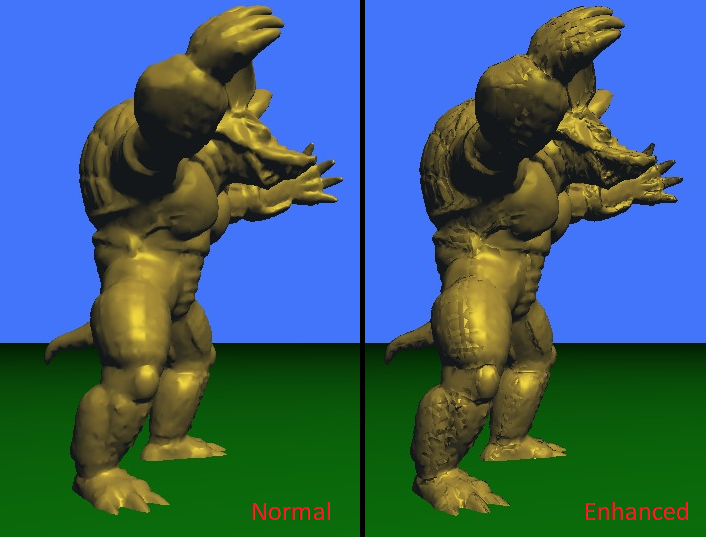
\includegraphics[width=0.8\textwidth]{Images/blinn_comparison.png}
	\caption{Comparison between standard Blinn-Phong and Enhanced Blinn-Phong using Geometry-based shading}
	\label{fig:blinn_comparison}
\end{figure}

\subsubsection{Enhanced Cartoon/Cel Shading implementation}
Lorem ipsum dolor sit amet, consectetur adipiscing elit. Aliquam fringilla fringilla dui id vehicula. Vestibulum aliquet, dui non viverra cursus, odio felis laoreet justo, ultricies blandit massa elit id lacus. Donec est lorem, aliquet ac gravida ac, egestas in elit. Sed sed ultrices tellus. Sed placerat nibh vel leo elementum, at aliquet turpis auctor. Etiam volutpat est risus, sit amet vehicula justo molestie sit amet. Donec fermentum libero in risus lobortis pellentesque. Sed dapibus, leo in congue dapibus, risus risus congue dolor, ac convallis lectus magna placerat ligula. Nam at turpis nisi. In scelerisque, libero vel laoreet tristique, est nunc maximus ipsum, non laoreet orci lorem ut dui. Cras vel est at ex congue congue sit amet id lectus. Nullam in tortor elementum, tempus eros vel, sagittis diam. Curabitur ultrices est nec est rhoncus malesuada. Mauris rhoncus nulla in ligula congue rhoncus. Suspendisse aliquet pellentesque lacus, nec varius neque sagittis et.
\subsubsection{Enhanced Gooch Shading implementation}
Lorem ipsum dolor sit amet, consectetur adipiscing elit. Aliquam fringilla fringilla dui id vehicula. Vestibulum aliquet, dui non viverra cursus, odio felis laoreet justo, ultricies blandit massa elit id lacus. Donec est lorem, aliquet ac gravida ac, egestas in elit. Sed sed ultrices tellus. Sed placerat nibh vel leo elementum, at aliquet turpis auctor. Etiam volutpat est risus, sit amet vehicula justo molestie sit amet. Donec fermentum libero in risus lobortis pellentesque. Sed dapibus, leo in congue dapibus, risus risus congue dolor, ac convallis lectus magna placerat ligula. Nam at turpis nisi. In scelerisque, libero vel laoreet tristique, est nunc maximus ipsum, non laoreet orci lorem ut dui. Cras vel est at ex congue congue sit amet id lectus. Nullam in tortor elementum, tempus eros vel, sagittis diam. Curabitur ultrices est nec est rhoncus malesuada. Mauris rhoncus nulla in ligula congue rhoncus. Suspendisse aliquet pellentesque lacus, nec varius neque sagittis et.
	\section{Conclusions}
Lorem ipsum dolor sit amet, consectetur adipiscing elit. Aliquam fringilla fringilla dui id vehicula. Vestibulum aliquet, dui non viverra cursus, odio felis laoreet justo, ultricies blandit massa elit id lacus. Donec est lorem, aliquet ac gravida ac, egestas in elit. Sed sed ultrices tellus. Sed placerat nibh vel leo elementum, at aliquet turpis auctor. Etiam volutpat est risus, sit amet vehicula justo molestie sit amet. Donec fermentum libero in risus lobortis pellentesque. Sed dapibus, leo in congue dapibus, risus risus congue dolor, ac convallis lectus magna placerat ligula. Nam at turpis nisi. In scelerisque, libero vel laoreet tristique, est nunc maximus ipsum, non laoreet orci lorem ut dui. Cras vel est at ex congue congue sit amet id lectus. Nullam in tortor elementum, tempus eros vel, sagittis diam. Curabitur ultrices est nec est rhoncus malesuada. Mauris rhoncus nulla in ligula congue rhoncus. Suspendisse aliquet pellentesque lacus, nec varius neque sagittis et.
\cite{lamport94}
	\bibliographystyle{IEEEtran}
	\begin{thebibliography}{9}
	\bibitem{texbook}
	Donald E. Knuth (1986) \emph{The \TeX{} Book}, Addison-Wesley Professional.
	
	\bibitem{lamport94}
	Leslie Lamport (1994) \emph{\LaTeX: a document preparation system}, Addison
	Wesley, Massachusetts, 2nd ed.
\end{thebibliography}
\end{document}